
\section{Perceived job risks predict realized job transitions} 

\subsection{Data}

The data on perceived job risks is derived from the Survey of Consumer Expectations (SCE) by the Federal Reserve Bank of New York. The SCE is a nationally representative online survey conducted with a rotating panel of approximately 1,300 household heads. The specific questions used to elicit perceived job finding and job separation probabilities are as follows: 
\begin{quote}
    \emph{What do you think is the percent chance that you will lose your main (for those with multiple jobs) or current (for those with single job) job during the next 12 months?}
\end{quote}

\begin{quote}
    \emph{Suppose you were to lose your main job this month, what do you think is the percent chance that you will find a job within the following 3 months?}
\end{quote}

The realized rates of job transitions are calculated using data from the Current Population Survey (CPS) \citep[e.g.,][]{fujita2009cyclicality}, which tracks the movement of workers between unemployment, employment, and non-participation statuses based on panel records of individual work histories. The job finding (${JF}_t$) and job separation (${JS}_t$) rates are defined as
\begin{equation*}
\label{eq:flow_rate_eq} 
JF_t=\frac{UE_t}{U_{t-1}}, \quad JS_t=\frac{EU_t}{E_{t-1}},
\end{equation*}
where $UE_t$ is the number of transitions from unemployment to employment in month $t$, $EU_t$ is the number of transitions from employment to unemployment in month $t$, $U_{t-1}$ is the number of individuals unemployed in month $t-1$, and $E_{t-1}$ is the number of individuals employed in month $t-1$. 
%\footnote{See \cite{Shimer:2005AER,fujita2009cyclicality} for the difference between gross-flow-based measures and duration-based measures.} 
We directly obtain the data on realized transition rates across various demographic groups, such as by education and income, from the labor market tracker provided by the Federal Reserve Bank of San Francisco.\footnote{Available at \url{www.frbsf.org/research-and-insights/data-and-indicators/sf-fed-data-explorer/}.} 


\paragraph{Time Aggregation.} The perceived transition probabilities are reported for different horizons from the realized flow rates. For consistency, we convert all these rates into 3-month horizons using the following procedure. Consider the flow rates for three consecutive months, denoted $p_1$, $p_2$, $p_3$. The aggregated flow rate over the 3-month window is then given by $1- (1-p_1)(1-p_2)(1-p_3)$. For the 1-year horizon job separation probability, we first convert it into a continuous-time Poisson rate and then re-convert it into a 3-month horizon. 


\subsection{Perceived risks versus realized outcomes}
\label{subsec:comparison_simple}

Figure \ref{fig:simple_comparison} directly compares perceived risks and realized job transitions for the sample period since 2013. It shows that perceptions predict realizations reasonably well at the aggregate level. This is evident not only in the similarity of the magnitudes of the two series but also in the highly positive correlation coefficients between them. Specifically, the 3-month-ahead perceived job-finding rate accounts for approximately 70\% of realized job transitions, while the perceived job-separation rate accounts for 37\% of its realization. 

\begin{figure}[!ht] \centering  % [h!]
	\caption{Perceived versus realized job transitions} 
	\label{fig:simple_comparison}
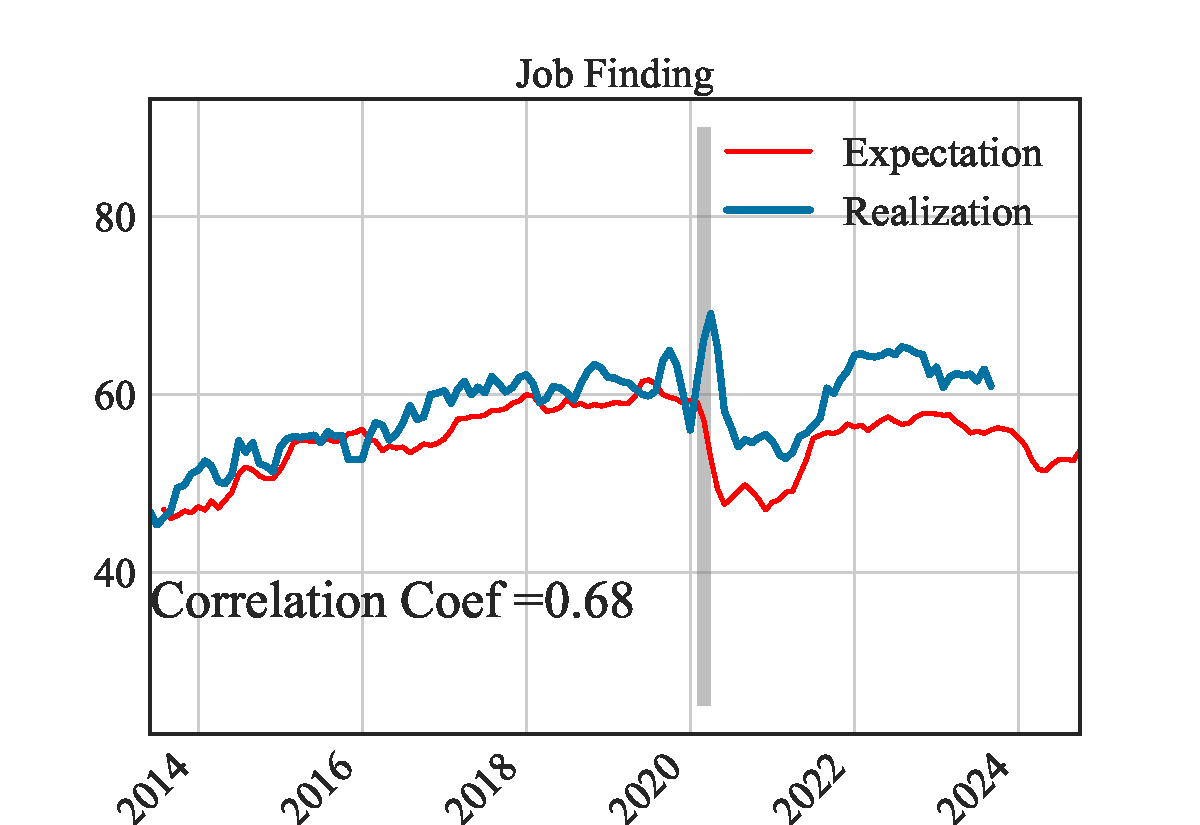
\includegraphics[width=0.49\linewidth]{text/chapter2/Figures/expectation_realization_comparison_JF.pdf} 
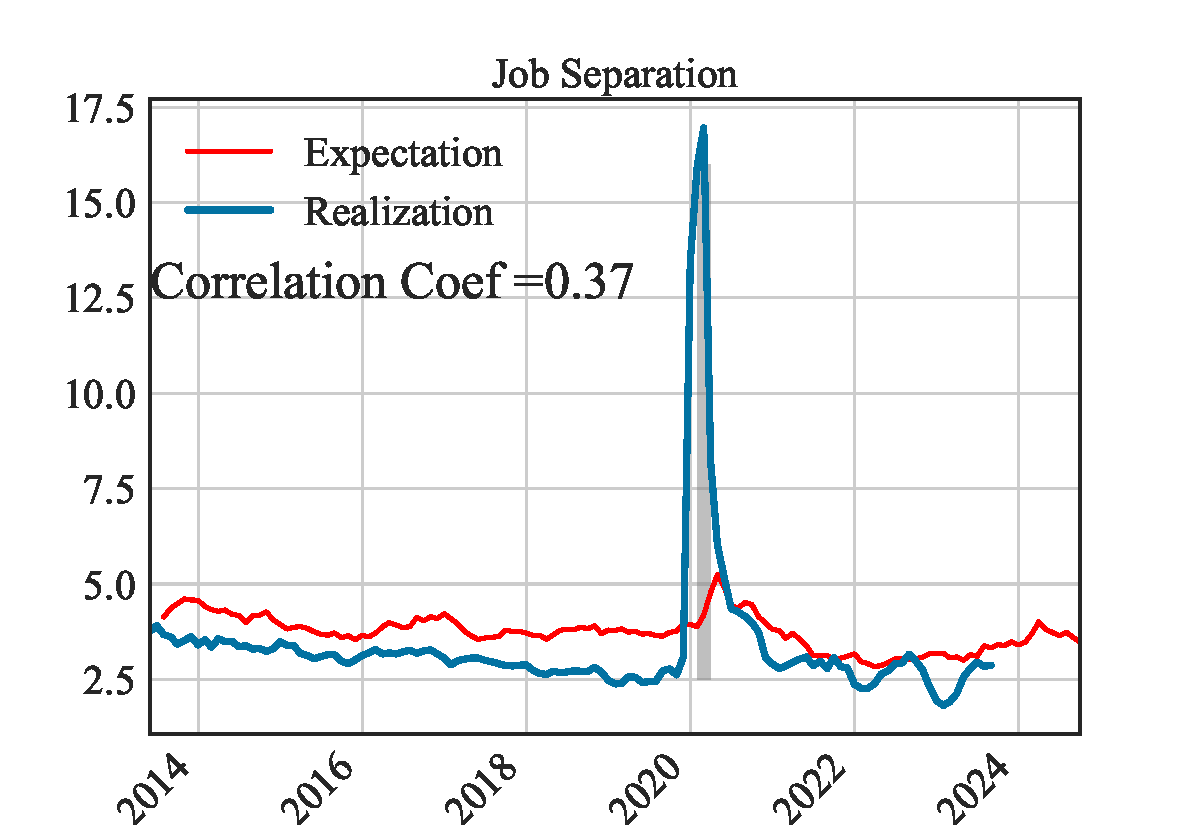
\includegraphics[width=0.49\linewidth]{text/chapter2/Figures/expectation_realization_comparison_JS.pdf} 
\floatfoot{\footnotesize{This figure plots the perceived job transition probabilities over next three months, $\widetilde{JF}_{t+3|t}$ and $\widetilde{JS}_{t+3|t}$ and the realized job flow rates three months later ${JF}_{t+3}$ and ${JS}_{t+3}$. All rates are in the units of percent chance.}}
\end{figure}


The correlation between perceived risks and realized flow rates would have been even higher without the COVID pandemic crisis, which introduced the most significant deviations of perceived risks from subsequent realizations. At the onset of the pandemic, the perceived job-finding rate dropped sharply, but the actual job-finding rate increased initially. This discrepancy was partly driven by the rehiring of previously laid-off workers through recalls. Similarly, while perceived separation risk spiked at the onset of the crisis, the spike was dwarfed by a much higher increase in the realized job separation rates. Such deviations highlight the unexpected nature of the COVID shock. However, the dynamics of perceived risks and corresponding realizations moved in tandem again within two months following the initial outbreak. The unusual labor market dynamics during the COVID crisis were unprecedented even for professional economists in real-time, and continue to be a subject of current and future studies. Therefore, it is noteworthy that average perceptions of job risks could still partially predict ex-post labor market flow rates, despite the unprecedented crisis.

The fact that perceived risk predicts subsequent changes in the labor market is, on one hand, surprising, and on the other hand, reassuring. Growing survey evidence suggests that households' macroeconomic expectations, especially regarding inflation and unemployment rates, tend to contain systematic forecast errors. However, the average perceived job risks reported based on individuals' situations appear to capture predictable movements in subsequent labor market flows. This is encouraging for our analysis of perceived job risks, as it suggests that these measured beliefs contain meaningful time variations that reflect the underlying state of the economy. On the other hand, the correlation between ex-ante perceived job risks and ex-post realized transitions, while positive, is far from perfect, indicating a deviation from perfect foresight. Regardless of what the ex-ante perceptions are, realized job flow rates inevitably incorporate the realization of ex-ante unexpected macroeconomic shocks or idiosyncratic shocks. 


\paragraph{Within-Group Comparison.} The results presented above are based on average rates across all households in the survey. One potential concern when generalizing these findings is how perceptions and realizations compare within demographic groups. Several studies such as \citet{hall2019job,gregory2021alpha,patterson2023matching} show the importance of heterogeneity in job risks in driving aggregate labor market dynamics, while \citet{broer2021information} provide indicative evidence that information frictions are heterogeneous along the wealth distribution. Therefore, we also calculate both perceptions and realizations separately for low, middle, and high education groups, separately, as plotted in Figure \ref{fig:simple_comparison_by_educ}. The figure reveals that, within each education group, the dynamics of perceived risk and realized rates closely mirror those observed at the aggregate level, exhibiting a high correlation during normal times. There is, however, substantial heterogeneity by education level in the realized rates, both in terms of overall levels and time-series volatility. Not surprisingly, low-education workers face higher job separation and lower job-finding rates than high-education ones. The differences in perceived job risks, especially in job separation rates, are relatively small across education groups. Interestingly, low-education workers appear to particularly underforecast their job separation rates at the onset of the pandemic, with the subsequent increase in separation rates being much larger than for the other two groups. Additionally, while low-education workers were notably more pessimistic about their job-finding prospects, the dynamics of realized job-finding rates were similar across all education groups. These patterns underscore the importance of considering heterogeneity in both the job risks faced by different groups and the perceptions of those risks. We explore these two points in the later part of the paper. 

\begin{figure}[pt] 
    \centering  
    \caption{Perceived versus realized job transitions: by education} 
    \label{fig:simple_comparison_by_educ}

    \begin{subfigure}{0.32\linewidth}
        \centering
        \caption{JF of Low Education}
        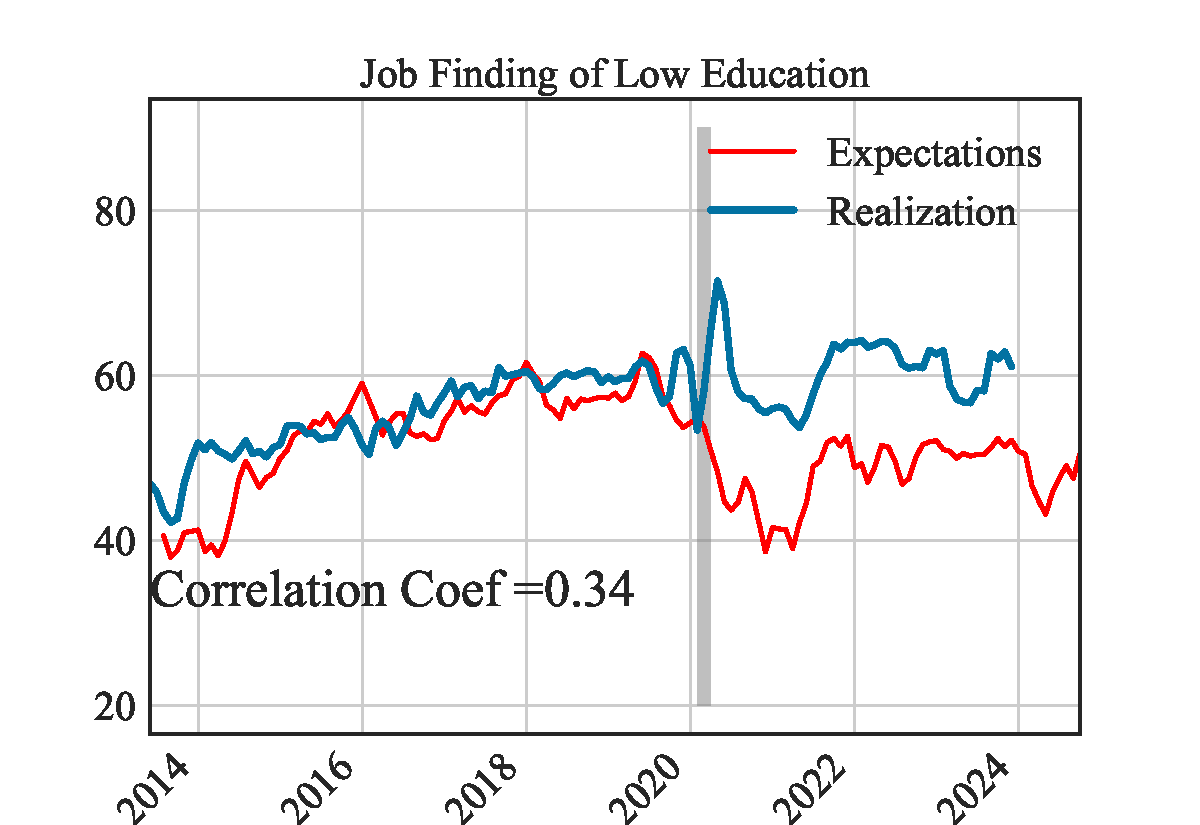
\includegraphics[width=\linewidth]{text/chapter2/Figures/expectation_realization_comparison_JF_LowEdu.pdf}  
        \label{fig:subfig1}
    \end{subfigure}
    \begin{subfigure}{0.32\linewidth}
        \centering
        \caption{JF of Middle Education}
        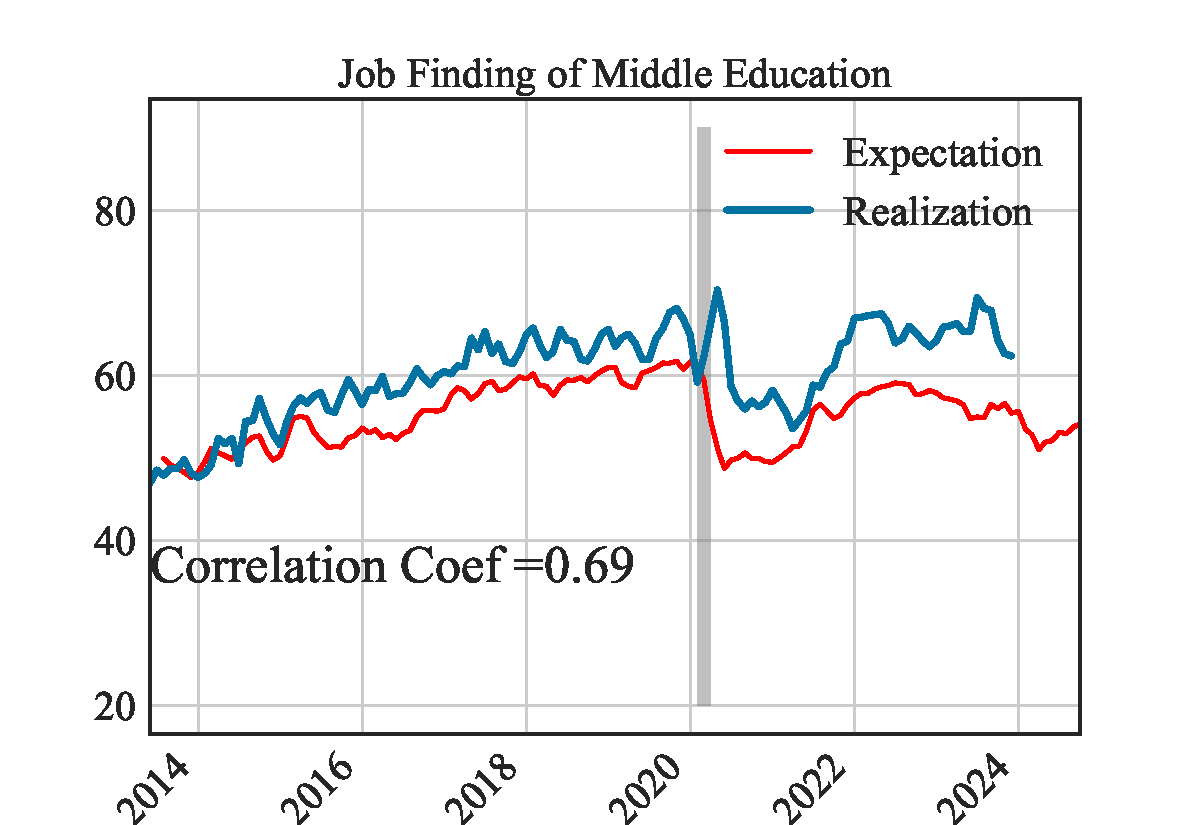
\includegraphics[width=\linewidth]{text/chapter2/Figures/expectation_realization_comparison_JF_MidEdu.pdf} 
        \label{fig:subfig2}
    \end{subfigure}
    \begin{subfigure}{0.32\linewidth}
        \centering
        \caption{JF of High Education}
        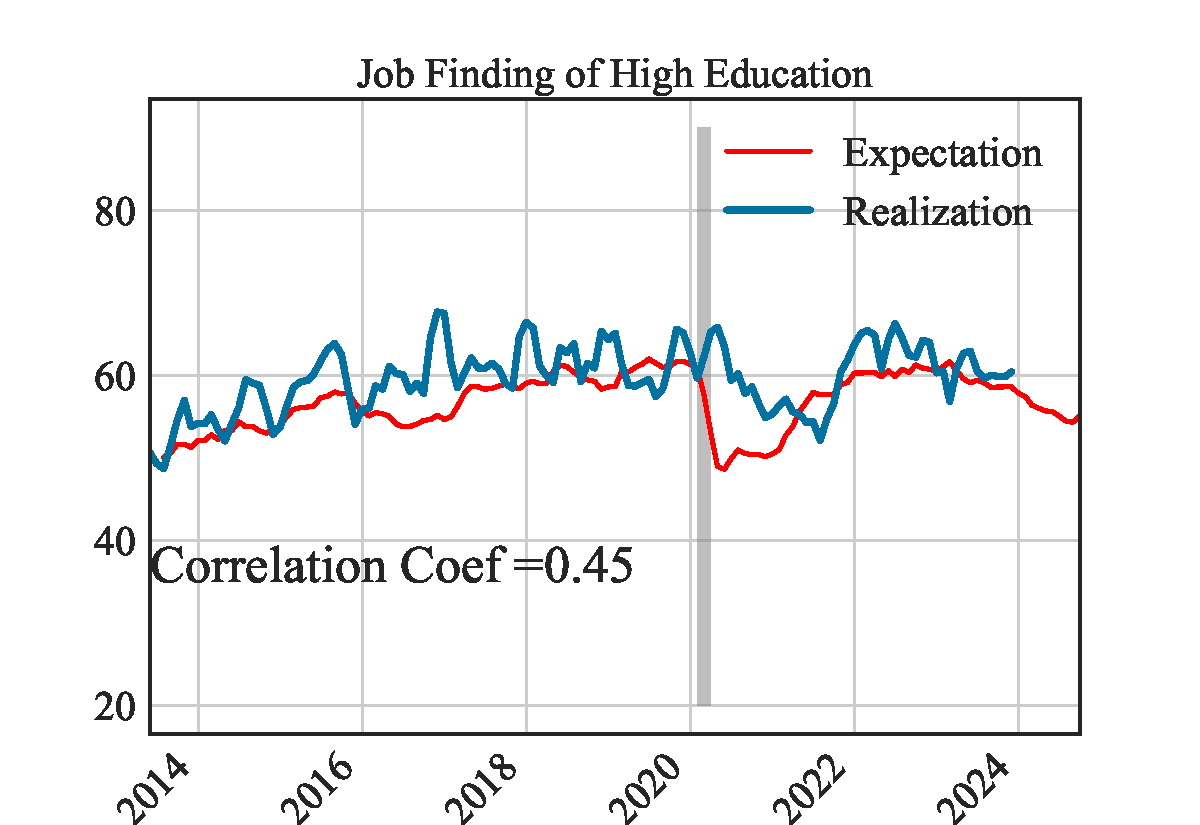
\includegraphics[width=\linewidth]{text/chapter2/Figures/expectation_realization_comparison_JF_HighEdu.pdf} 
        \label{fig:subfig3}
    \end{subfigure}

    \begin{subfigure}{0.32\linewidth}
        \centering
        \caption{JS of Low Education}
        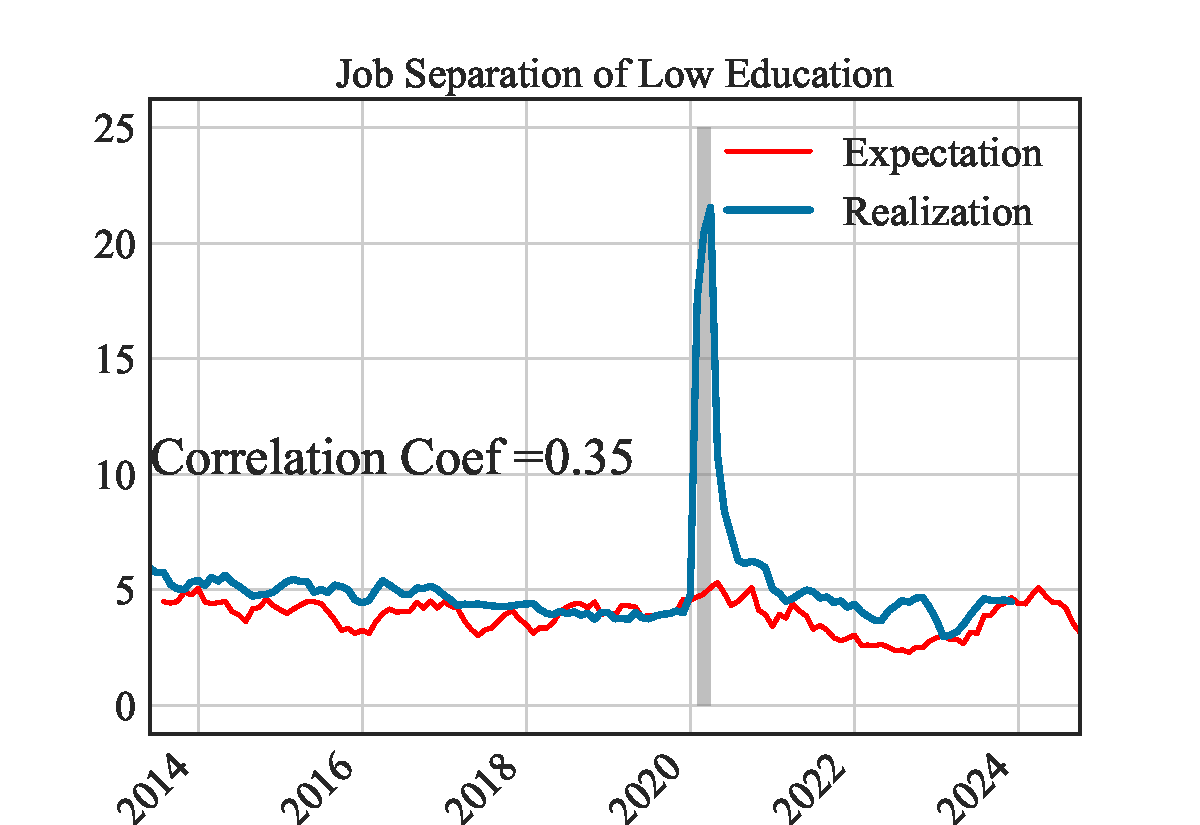
\includegraphics[width=\linewidth]{text/chapter2/Figures/expectation_realization_comparison_JS_EduLow.pdf}  
        \label{fig:subfig4}
    \end{subfigure}
    \begin{subfigure}{0.32\linewidth}
        \centering
        \caption{JS of Middle Education}
        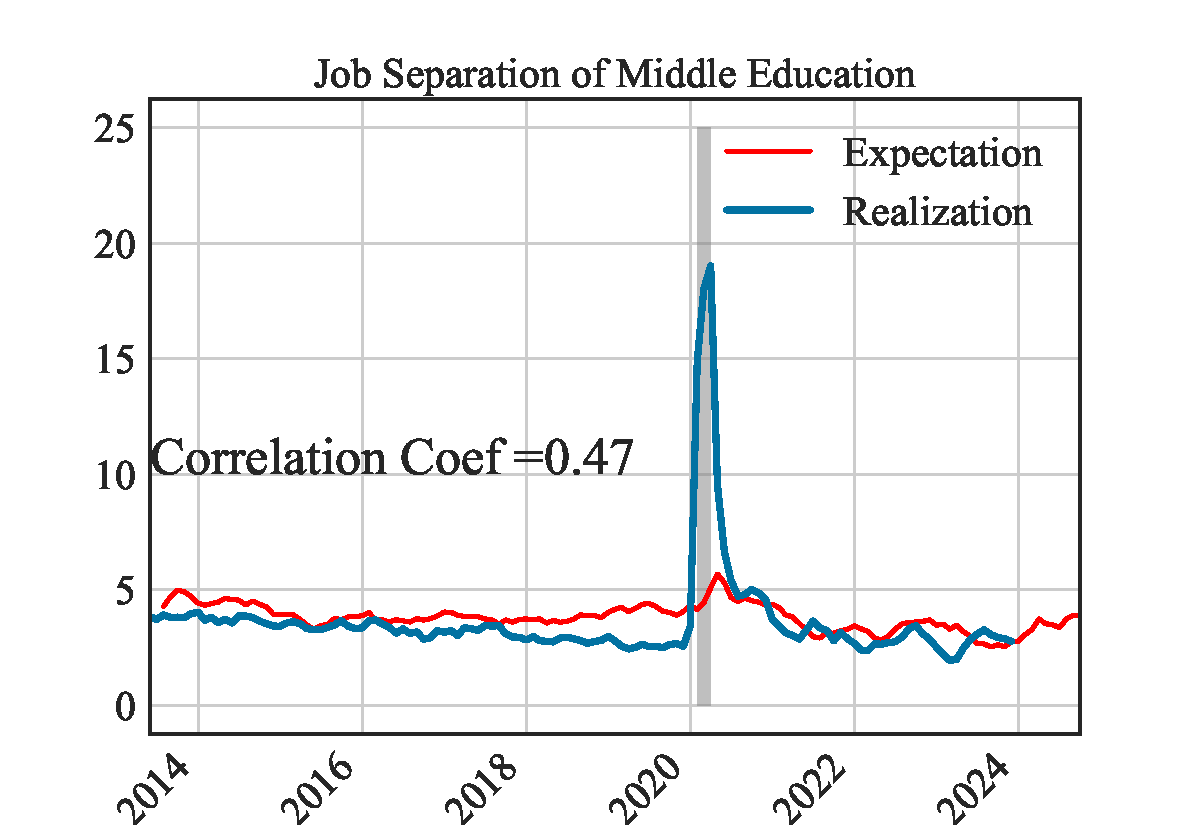
\includegraphics[width=\linewidth]{text/chapter2/Figures/expectation_realization_comparison_JS_EduMid.pdf} 
        \label{fig:subfig5}
    \end{subfigure}
    \begin{subfigure}{0.32\linewidth}
        \centering
        \caption{JS of High Education}
        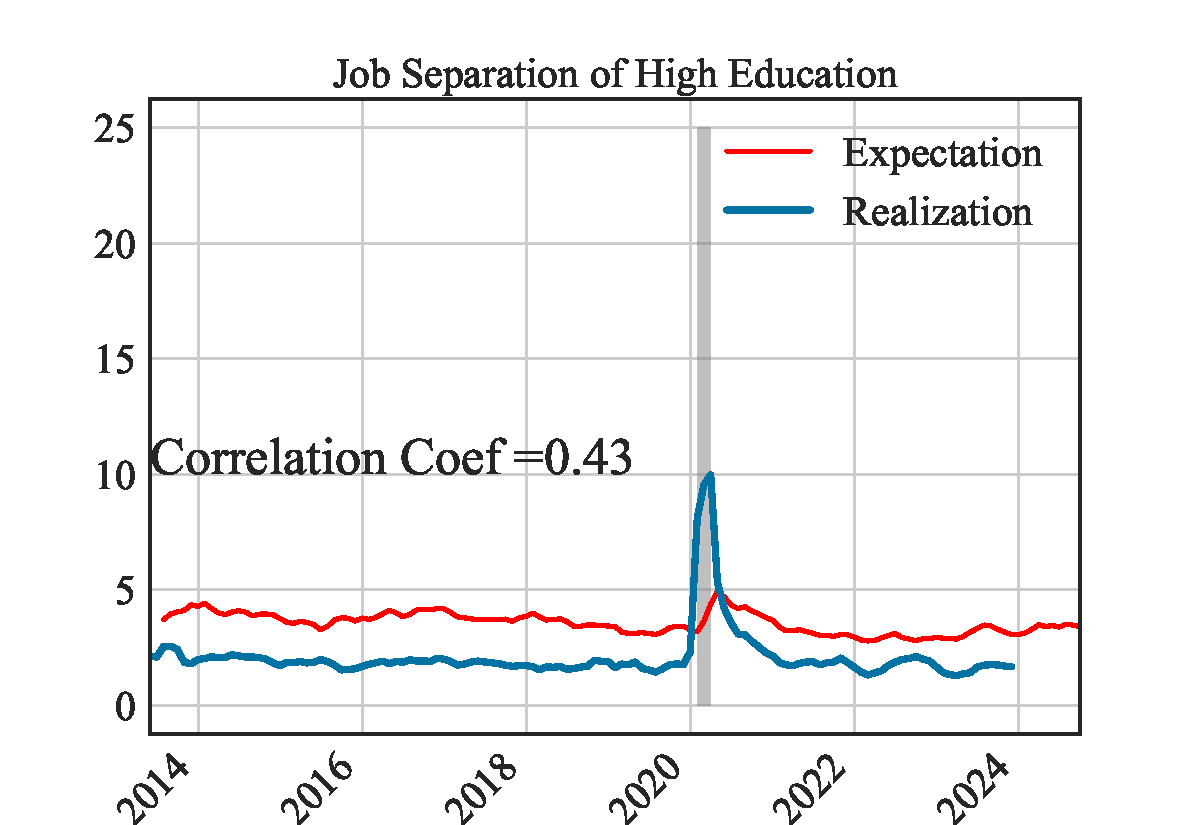
\includegraphics[width=\linewidth]{text/chapter2/Figures/expectation_realization_comparison_JS_EduHigh.pdf} 
        \label{fig:subfig6}
    \end{subfigure}

    \floatfoot{\footnotesize{This figure plots the 3-month-ahead job risk expectations, measured as perceived job finding and separation rates in SCE, by different education groups, $\widetilde{JF}^{Educ}_{t+3|t}$ and $\widetilde{JS}^{Educ}_{t+3|t}$ $\forall {Educ} \in \{High, Mid, Low\}$, along with their respective realization 3 months later obtained from the San Francisco Fed, ${JF}^{Educ}_{t+3}$ and ${JS}^{Educ}_{t+3}$ $\forall{Educ} \in \{High, Mid, Low\}$. All rates are in the units of percent chance.}}
\end{figure}


%Regardless of the differences between the two series of realized job-finding rates, there is one common pattern in the imputed belief series compared to its realizations: the belief is less volatile than realizations throughout the entire period. One obvious interpretation of this pattern is that belief does not react to aggregate labor market changes as much as it turned out to be. This is reminiscent of the underreaction/stubbornness in expectation-formation as modeled in \cite{menzio2022stubborn}.\footnote{Such a mechanism has been modeled and supported by empirical evidence mostly in other  contexts: information rigidity as in \cite{coibion2015information}, or sticky expectation model as in xxx.}

\subsection{Forecast errors of perceived job risks}

To systematically assess the relationship between perceived risks and realized job transitions, we adopt a widely used metric in the literature: forecast errors (FE), defined as the difference between the perceived risk and realized flow rate. 
\begin{equation}
\text{FE}^{JF}_{t,t+3} = \widetilde{\text{JF}}_{t+3|t} - \text{JF}_{t,t+3}  ,
\end{equation}
where the expectation is formed over a 3-month horizon. Here, $\widetilde{\text{JF}}_{t+3|t}$ represents the perceived job-finding rate for 3 months ahead at time $t$ and $\text{JF}_{t,t+3}$ is the realization over the same horizon.

To test the informational efficiency of perceived job risks, we perform a 3-month-apart auto-regression of forecast errors with an intercept term, which is commonly used in the literature on expectation formation, e.g., \cite{coibion2015information}, \cite{fuhrer2018intrinsic}, and \cite{coibion2018firms}.
\begin{equation}
\label{eq:forecast_error_autoreg}
\text{FE}^{JF}_{t,t+3} = \alpha + \beta \text{FE}^{JF}_{t-3,t} + \gamma X_{t-3} +\epsilon_t ,
\end{equation}
where $X_{t-3}$ denotes information available at time $t-3$. A key null hypothesis under FIRE is that agents do not fully react to new shocks to the underlying variable. A significantly positive $\beta$ implies predictable forecast errors based on past forecast errors.\footnote{A related null hypothesis in the same spirit is based on a regression of forecast errors on past information $X_{t-3}$, which states that $\gamma$ being statistically different from zero means information available at $t-3$ predicts future forecast errors, implying that they are not fully utilized when the forecasts are made. We provide additional results of such tests in the Appendix \ref{appendix:fe_results_more}.} In particular, $\beta>0$ suggests that past errors persist into future forecasts in the same direction, reflecting the presence of information rigidity. 

\begin{table}[!htbp] \centering
  \caption{Forecast Error Regression}
  \label{tab:fe_regression}
  \begin{adjustbox}{width=\textwidth}
\begin{tabular}{@{\extracolsep{5pt}}lcccccccc}
\\[-1.8ex]\hline
\hline \\[-1.8ex]
\\[-1.8ex] & \multicolumn{1}{c}{JF} & \multicolumn{1}{c}{JF LowEdu} & \multicolumn{1}{c}{JF MidEdu} & \multicolumn{1}{c}{JF HighEdu} & \multicolumn{1}{c}{JS} & \multicolumn{1}{c}{JS LowEdu} & \multicolumn{1}{c}{JS MidEdu} & \multicolumn{1}{c}{JS HighEdu}  \\
\hline \\[-1.8ex]
 Constant & -0.027$^{***}$ & -0.027$^{***}$ & -0.038$^{***}$ & -0.024$^{***}$ & 0.003$^{*}$ & 0.076$^{***}$ & 0.079$^{***}$ & 0.051$^{***}$ \\
  & (0.004) & (0.007) & (0.005) & (0.004) & (0.002) & (0.009) & (0.010) & (0.009) \\
 lag\_FE\_jf & 0.256$^{***}$ & 0.545$^{***}$ & 0.272$^{***}$ & 0.183$^{**}$ & & & & \\
  & (0.087) & (0.076) & (0.084) & (0.088) & & & & \\
 lag\_FE\_js & & & & & 0.131$^{}$ & 0.202$^{**}$ & 0.267$^{***}$ & 0.554$^{***}$ \\
  & & & & & (0.091) & (0.089) & (0.088) & (0.075) \\
\hline \\[-1.8ex]
 Observations & 121 & 124 & 124 & 124 & 121 & 124 & 124 & 124 \\
 $R^2$ & 0.068 & 0.295 & 0.079 & 0.034 & 0.017 & 0.040 & 0.070 & 0.308 \\
 Adjusted $R^2$ & 0.060 & 0.289 & 0.071 & 0.026 & 0.009 & 0.032 & 0.062 & 0.302 \\
 F Statistic & 8.628$^{***}$  & 51.049$^{***}$  & 10.452$^{***}$  & 4.297$^{**}$  & 2.062$^{}$  & 5.103$^{**}$  & 9.197$^{***}$  & 54.322$^{***}$  \\
\hline
\hline \\[-1.8ex]
 & \multicolumn{8}{r}{$^{*}$p$<$0.1; $^{**}$p$<$0.05; $^{***}$p$<$0.01} \\
\end{tabular}
\end{adjustbox}
\floatfoot{\footnotesize{The table reports the auto-regression results of average and various education groups' respective average forecast errors of expectations of job finding and separation rate with their respective 3-month-lagged values, as defined in Equation \ref{eq:forecast_error_autoreg}.}}
\end{table}

The estimation results for forecast errors in job-finding and separation perceptions are reported in Table \ref{tab:fe_regression}. They overwhelmingly reject the null hypothesis of full efficiency ($\beta=0$). Specifically, the 3-month-apart auto-regression coefficient of average forecast errors in job-finding is 0.256. Education-specific estimates range from 0.183 for the high-education group to 0.535 for the low-education group. For job separation, although the auto-correlation of average forecast errors is not significant, forecast errors of education-specific perceptions all show significantly positive auto-correlations, with regression coefficients ranging from 0.20 for the low-education group to 0.55 for the high-education group. 

These estimates of auto-correlation of non-overlapping forecast errors suggest the presence of information rigidity in perceived job transition risks. However, the fact that the estimates are not close to one indicates that the information rigidity is moderate. This is particularly the case if the shocks to job finding and separation are relatively persistent, which means that only a mild degree of information rigidity sufficiently leads to non-zero auto-correlation of forecast errors. 

Besides a non-zero serial correlation of forecast errors, as revealed in estimated $\beta$, it is worth noting that the constant term $\alpha$ in the auto-regression is also informative. Under FIRE, a positive (negative) $\alpha$ indicates an upward (downward) bias in the average forecasts. Its estimates in Table \ref{tab:fe_regression} are significantly different from zero. Forecast errors of job-finding perceptions are on average positive and that of job separation is negative. At face value, this implies that ex-ante perceptions of job risks underestimates the job finding, and overforecasts the job separation rates. Although it is tempting to conclude that job risk perceptions are biased based on such evidence, as argued in several papers, we only focus in this paper on the dynamic rigidity of risk perceptions instead of its constant bias in levels with a cautionary note that the sign of the latter is sensitive to the exact procedure of aggregation of individual beliefs.\footnote{\cite{arni2013s}, \cite{conlon2018labor}, \cite{mueller2021job}, based on a comparison of average survey perceptions and realization, concluded that workers over perceive job finding probability. Meanwhile, \cite{stephens2004job}, \cite{dickerson2012fears}, \cite{balleer2023biased} found that workers overperceive job separation probabilities relative to their realizations.} 